\chapter{Grundlagen}

\section{Physikalische Konzepte}
    \subsection{Kristallstrukturen im Festkörper}
        \subsubsection{Kubische Gitter}

\begin{figure}[h]
    \centering
    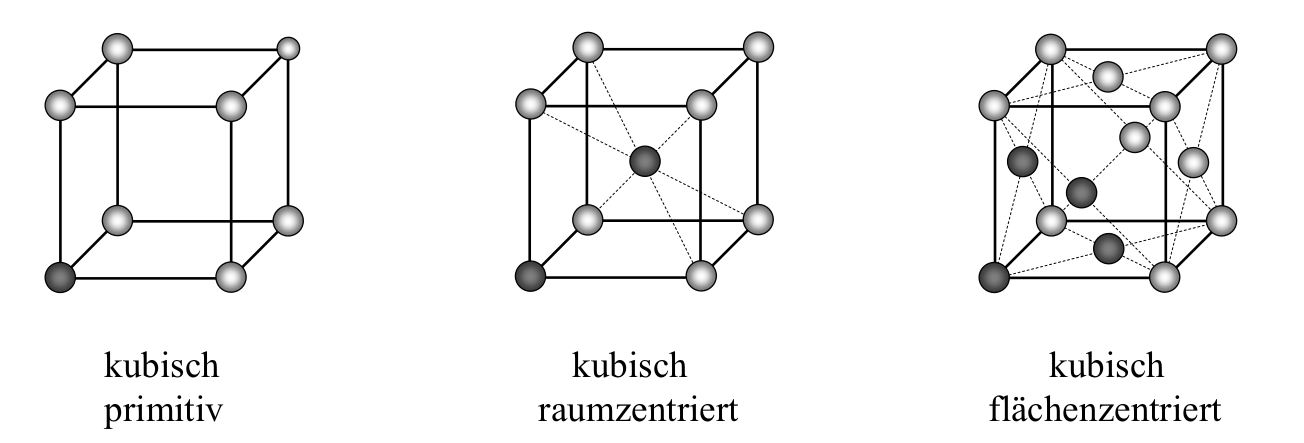
\includegraphics[width=0.9\textwidth]{Abb/kubische_gitter.png}
    \caption{Die drei kubischen Atomgitter. Von links nach rechts: 
             einfach kubisch (sc), kubisch raumzentriert (bcc),
             kubisch flächenzentriert (fcc) \cite{hunklinger}}
    \label{kub}
\end{figure}
Es existieren drei verschiedene kubische Gitter.
Diese sind in Abbildung \ref{kub} dargestellt. Im Rahmen dieses Versuches
soll nur das kubisch flächenzentrierte Gitter näher betrachtet werden. Viele Metalle
und Legierungen kristallisieren in diese Anordnung.\\
\begin{figure}
    \centering
    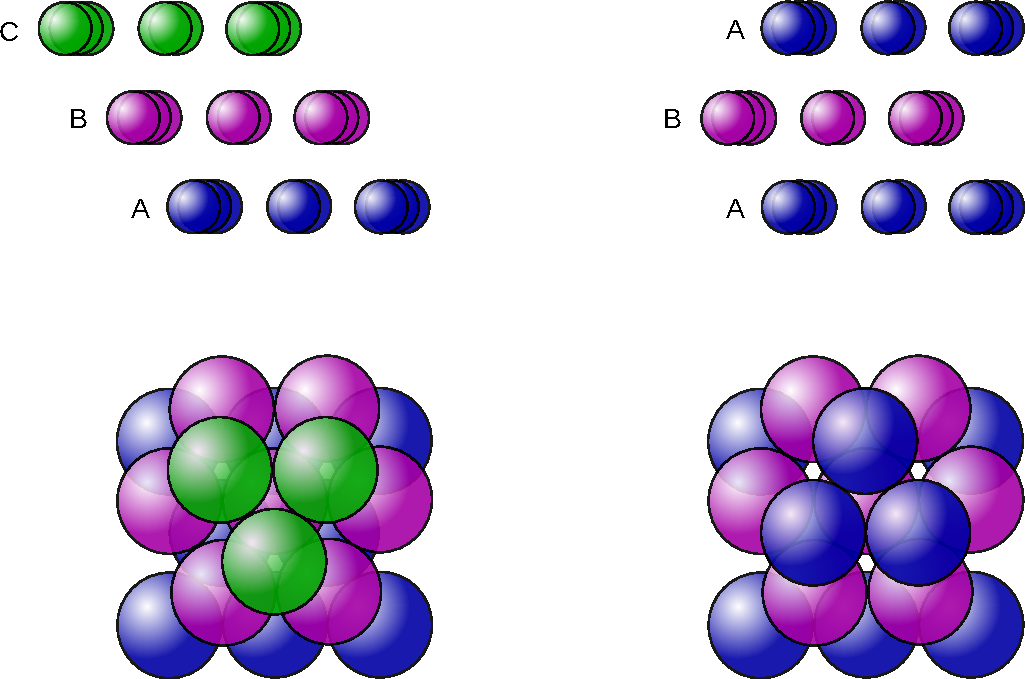
\includegraphics[width=0.7\textwidth]{Abb/DichtesteKugelpackung.pdf}
    \caption{Die möglichen Stapelfolgen für eine dichteste Kugelpackung:
             Links im Bild werden drei verschiedene Schichten gestapelt,
             also ABCABC... 
             Rechts werden nur zwei Schichten gestapelt, die dritte Schicht liegt
             also exakt auf der Ersten, ABABAB... \cite{kugel}}
    \label{pack}
\end{figure}
Betrachtet man eine möglichst dichte Packung an Kugeln, so sind zwei Stapelfolgen 
möglich. Das fcc-Gitter repräsentiert hierbei die Schichtfolge ABCABC..., siehe 
hierzu Abbildung \ref{pack}. Ein Atom hat in dieser Anordnung 12 nächste Nachbarn
mit dem Abstand $\frac{a}{\sqrt{2}}$. $a$ sei hier die Gitterkonstante des Würfels.
In einer kubischer Zelle befinden sich $8 \cdot \frac{1}{8} + 6 \cdot \frac{1}{2} 
= 4$ Atome. Die Atome an den Ecken befinden sich in acht Zellen gleichzeitig, jene 
an den Flächen in zwei. Sie werden deshalb anteilig hinzugerechnet.
Die Packungsdichte $ V_{\text{Atome}} / V_{\text{kub. Zelle}} $ ergibt sich somit zu:
\[
    \underset{\text{Volumen eines Atoms}}{
        \underbrace{
            \frac{4}{3} \left( \frac{d_{NN}}{2} \right)^2 \pi}} \cdot
    \underset{\text{Atome pro kubischer Zelle}}{4} 
    / \, 
    \underset{\text{Volumen des Würfels}}{a^3} \approx 0.74
\]
Die dichtest mögliche Kugelpackung nimmt also $74\%$ des Raums ein.

        \subsubsection{Hexagonal dichteste Kugelpackung}

\begin{wrapfigure}{r}{0.45\textwidth}
    \centering
    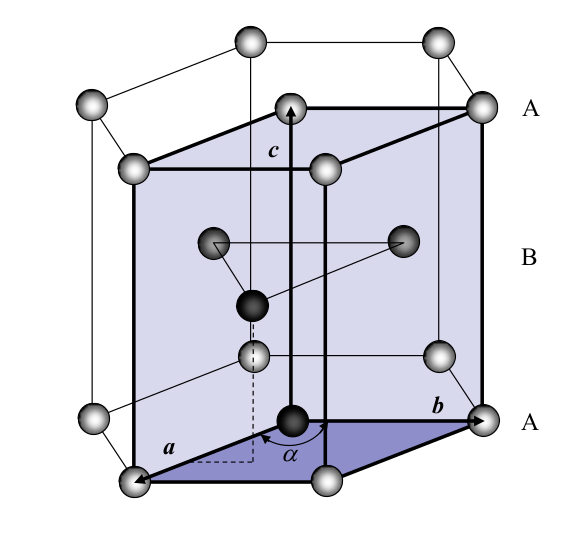
\includegraphics[width=0.4\textwidth]{Abb/hcp.png}
    \caption{hcp-Gitter \cite{hunklinger}}
    \label{hcp}
\end{wrapfigure}
Die rechte Stapelfolge in Abbildung \ref{pack} wird als hexagonal dichteste
Kugelpackung (hcp) bezeichnet. In Eigenschaften wie Abstand und Anzahl der nächsten
Nachbarn gleicht es dem fcc, was durch die Betrachtung als dichteste Packungen 
schnell klar wird. In Abbildung \ref{hcp} sind die Stapelfolgen eingezeichnet.
Die Vektoren $a$ und $b$ sind gleich lang. Für $c$ findet man $c = \sqrt{ 
\frac{8}{3}} \, a$. In realen Kristallen weicht dies oft etwas ab.

        \subsubsection{Graphenstruktur}

\begin{figure}
    \centering
    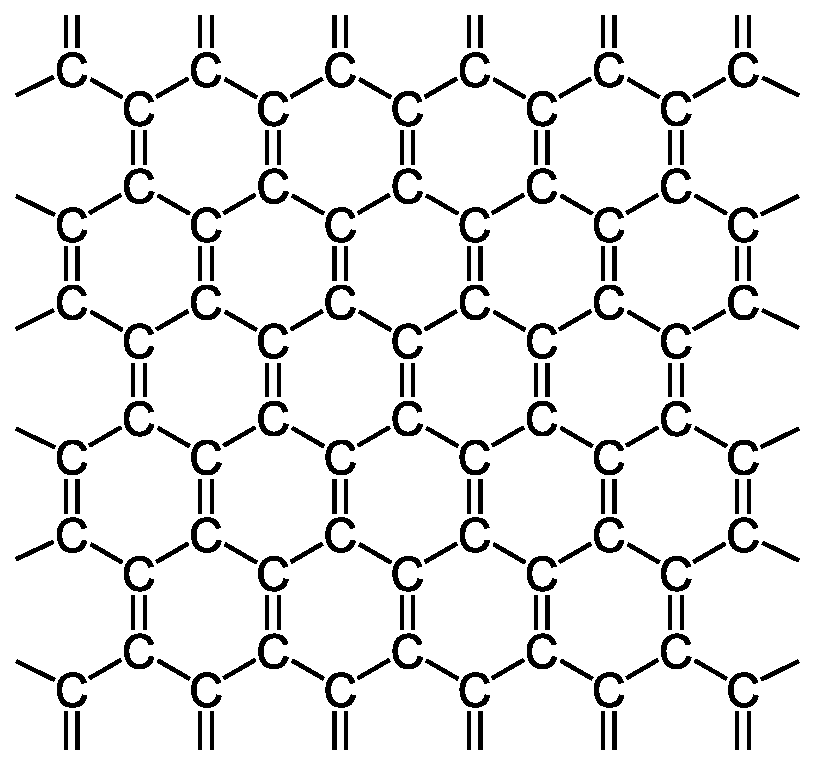
\includegraphics[width=0.4\textwidth]{Abb/graphenstruktur.pdf}
    \caption{Struktur von Graphen \cite{wikigraphen}}
    \label{graphenstruktur}
\end{figure}
In Abbildung \ref{graphenstruktur} ist die Bienenwabenstruktur des Graphens 
dargestellt. Es handelt sich um eine Atomlage von Kohlenstoffatomen, die durch
sp2-Hybridorbitale verbunden sind. Alle Bindungen sind hierbei gleich lang.
\cite{hunklinger}

    \subsection{Quantenmechanischer Tunneleffekt}

Das Tunneln beschreibt ein quantenmechanischen Effekt, nach dem es für Teilchen
möglich ist eine Energiebarriere zu überwinden, auch wenn diese eine wesentlich
höhere Energie als das Teilchen besitzt. Klassisch wäre dies unmöglich.\\
Wir betrachten eine Potentialbarriere 
\[
    V(x) = V_0 \Theta ( a - |x| )    
\]
und ein Teilchen mit der Energie $E < V_0$.
\begin{figure}[h]
   \centering
   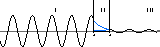
\includegraphics[width=0.9\textwidth]{Abb/tunnel.pdf}
   \caption{Skizze des Tunneleffekts: Die Wellenfunktion des Teilchens läuft von 
            links auf die Potentialbarriere zu. Nach einem exponentiellen Abfall
            im Inneren der Barriere besteht eine kleine Wahrscheinlichkeit, dass
            sich das Teilchen rechts der Barriere aufhält}
   \label{tunnel} 
\end{figure}
Benutzt man die stationäre Schrödingergleichung
\[
    - \frac{\hbar^2}{2m} \frac{d^2}{dx^2} \Phi(x) + V(x) \Phi(x) + V(x) \Phi(x)
    = E \Phi(x)    
\]
so findet sich für die Teilchenwellenfunktion
\[
    \Psi(x) = 
        \begin{cases}
            A \, e^{ikx} + B \, e^{-ikx}, \quad x<-a\\
            C \, e^{-\kappa x} + D \, e^{\kappa x} \quad -a < x < a\\
            F \, e^{ikx} + G \, e^{-ikx}, \quad x<-a
        \end{cases}
\]
mit den Wellenzahlen $k=\sqrt{2mE}/\hbar$ und $\kappa = \sqrt{2m(V_0-E)}/\hbar$.
Benutzt man nun die Anschlussbedingungen
\begin{align*}
    &x=-a: \quad A \, e^{-ika} + B \, e^{ika} = C \, e^{\kappa a} 
        + D \, e^{-\kappa a}\\
    &x=a: \quad F \, e^{+ika} + G \, e^{-ika} = C \, e^{-\kappa a} 
        + D \, e^{+\kappa a}
\end{align*}
und die Normalisierungsbedingung
\[
    \int \Psi^* (x) \Phi (x) dx = 1
\]
so kann man Ausdrücke für die einzelnen Koeffizienten erhalten. Für ein von links 
einfallendes Teilchen, also $G=0$, errechnet sich die Transmissionsamplitude 
$S(E)$ zu
\[
    S(E) = \frac{F}{A} = \frac{e^{-2ika}}{\cosh(2\kappa a) + \frac{i \varepsilon}{2}
                               \sinh(2\kappa a)}
\]
Die Wahrscheinlichkeit einer Transmission, der Durchlässigkeitskoeffizient, 
errechnet sich dann zu
\[
    | S(E) |^2 = \frac{1}{1+(1+(\varepsilon^2/4)) \, \sinh^2(2\kappa a)}
\]
Nimmt man nun eine sehr hohe und breite Barriere an, also $\kappa a >> 1$ und 
vernachlässigt die aus dieser Näherung resultierenden Logarithmusterme, so erhält
man den handlichen Ausdruck
\[
    | S(E) |^2 = \exp\left(-4 \sqrt{2m(V_0-E)} \, \frac{a}{\hbar}\right)
\]
\cite{schwabl}
% Tunneleffekt im STM fehlt noch
\newpage

    \subsection{Piezoelektrischer Effekt}

\begin{wrapfigure}{r}{0.3\textwidth}
    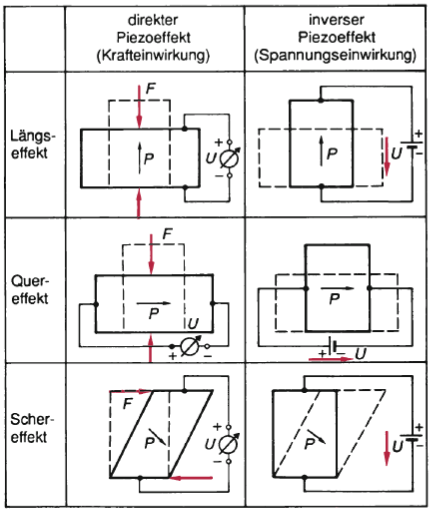
\includegraphics[width=0.3\textwidth]{Abb/piezo.png}
    \caption{Piezoelektrizität \cite{phying}}
    \label{piezo}
\end{wrapfigure}
Bestimmte Materialien erzeugen eine elektrische Spannung, sobald eine äußere Kraft
auf den Körper wirkt. Dies wird als piezoelektrischer Effekt bezeichnet. Er wurde
1880 durch die Brüder Curie an einigen Kristallen entdeckt.\\
Essentiell für die Rastersondenmikroskopie ist der inverse piezoelektrische Effekt.
Dieser führt zu einer Geometrieänderung des Kristalls beim Anlegen einer äußeren 
Spannung. Dies ermöglicht sehr feine Ortsänderungen der Spitze. Es werden drei 
technische nutzbare Vorgänge unterschieden, die in Abbildung \ref{piezo} skizziert
werden.
\begin{itemize}
    \item Längs-Effekt:\\
          Eine äußere Kraft $\textbf{F}$ führt zu einer Polarisierung $\textbf{P}$.
          Die resultierende Spannung $U$ liegt in gleicher Richtung an.
    \item Querr-Effekt:\\
          Eine äußere Kraft $\textbf{F}$ führt zu einer transversalen Polarisation
          $\textbf{P}$. Die resultierende Spannung $U$ liegt nun quer an.
    \item Scher-Effekt:\\
          Eine äußere Kraft $\textbf{F}$ führt zu einer diagonalen Polarisation
          $\textbf{P}$. Die resultierende Spannung $U$ liegt wiederum quer an.
\end{itemize}
Die Anwendungen der Piezoelektrizität sind weitreichend. Abbildung \ref{piezo_anw} 
gibt hierzu eine Übersicht. \cite{phying}
\begin{figure}[hb]
    \centering
    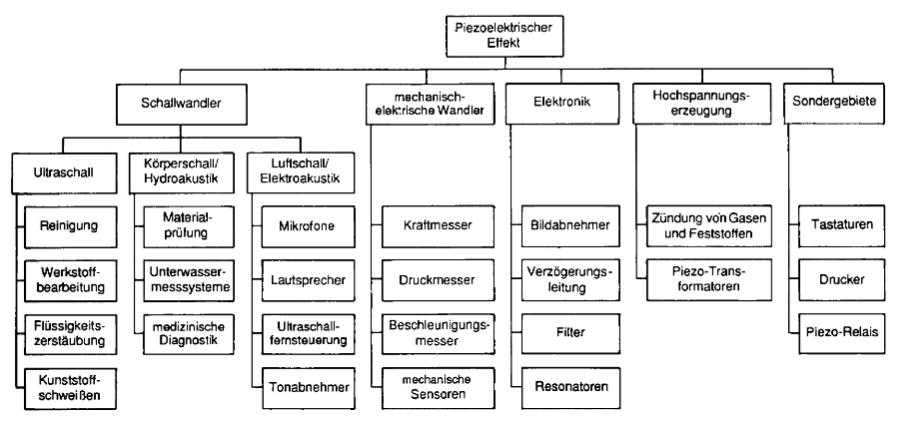
\includegraphics[width=0.9\textwidth]{Abb/piezo_anw.png}
    \caption{Anwendung der Piezoelektrizität \cite{phying}}
    \label{piezo_anw}
\end{figure}

\section{Aufbau eines Rastertunnelmikroskops}
    \subsection{Aufbau der Spitze}
    \subsection{Herstellung der Spitze}
    \subsection{Piezomotoren}

\section{Betriebsarten eines Rastertunnelmikroskops}
    \subsection{Topographischer Modus}
    \subsection{Modus konstanter Höhe}
    \subsection{Spektroskopie}

\section{Probenmaterialien}
    \subsection{Graphit}
    \subsection{Gold}
    \subsection{Molybdänsulfit}
